\documentclass[a4paper, 14pt]{extarticle}

% file's preambule

% Если вы работаете не в XeLaTeX, то сами разбирайтесь =)

% connect packages
%%%%%%%%%%%%%%%%%%%%%%%%%%%%%%%%%%%%%%%%%%%%%%%%%%%%%%%%%%%%%%%%%%%%%%
%\usepackage[T2A]{fontenc}                   %!? закрепляет внутреннюю кодировку LaTeX
%\usepackage[utf8]{inputenc}                 %!  закрепляет кодировку utf8
\usepackage{fontspec}                        % Шрифты
\usepackage{indentfirst}                    %   добавить indent перед первым параграфом
\setlength{\parindent}{1.27cm}
\usepackage{polyglossia}                     % Русский язык
\setdefaultlanguage{russian}
\setmainfont[Ligatures=TeX]{Times New Roman}
\newfontfamily\cyrillicfont{Times New Roman}[Script=Cyrillic]
%\usepackage[english,russian]{babel}         %!  подключает русский и английский
\usepackage{amsmath}                        %!  |
\usepackage{amssymb,textcomp, esvect,esint} %!  |важно для формул 
\usepackage{geometry}                       %!  отступ от граней
\geometry{verbose,a4paper,tmargin=2cm,bmargin=2cm,lmargin=3cm,rmargin=1cm}
\usepackage{amsfonts}                       %!  математические шрифты
\usepackage{amsthm}                         %!  newtheorem и их сквозная нумерация
\usepackage{graphicx}                       %?  графическое изменение текста
\usepackage{soulutf8}% Поддержка переносоустойчивых подчёркиваний и зачёркиваний
\usepackage{enumitem}                       %!  задание макета перечня.
%\usepackage[unicode, pdftex]{hyperref}      %!  оглавление для панели навигации по PDF-документу + гиперссылки
\usepackage{setspace}                       % Межстроковые интервалы
\onehalfspacing
\usepackage{booktabs}                       %!  добавляет книжные линии в таблицы
%\usepackage{hypcap}                         %?  адресация на картинку, а не на подпись к ней
\usepackage{abraces}                        %?  фигурные скобки сверху или снизу текста
\usepackage{caption}                        %-  позволяет корректировать caption 
\DeclareCaptionLabelSeparator{dash}{ - }
\captionsetup[table]{labelformat=simple, labelsep=dash, justification=raggedleft,
singlelinecheck=off}
\captionsetup[figure]{labelformat=simple, labelsep=dash}
\usepackage{multirow}                       %   объединение ячеек в таблицах
\usepackage{longtable}
\usepackage{pifont}                         %!  нужен для крестика
\usepackage{cancel}                         %!  аутентичное перечеркивание текста
\usepackage{ulem}                           %!  перечеркивание текста
\usepackage{tikz}                           %!  высокоуровневые рисунки (кружочек)
\usepackage{titling}                        %-  автоматическое заглавие 
\usepackage{titlesec}  % нормальные заголовки секций
\titleformat{\section}
{\normalfont\large\bfseries\filcenter}{}{1em}{}
\titleformat{\subsection}
  {\normalfont\normalsize\bfseries}{\thesubsection.}{5pt}{}
\titleformat{\subsubsection}
  {\normalfont\normalsize\bfseries}{\thesubsubsection.}{5pt}{}
\titleformat{\paragraph}
  {\normalfont\normalsize\bfseries}{\theparagraph}{5pt}{}

\usepackage{ragged2e} % Для выравнивания текста по ширине
\justifying

%\renewcommand{\thesubsubsection}{\alph{subsubsection}}
\usepackage{blindtext}                      %-  слепой текст
\usepackage{fancyhdr}                       %   добавить верхний и нижний колонтитул
\usepackage{mathptmx}

\usepackage{import}                         %|
\usepackage{xifthen}                        %|
\usepackage{pdfpages}                       %|
%\usepackage{transparent}                    %| вставка ink figures
\usepackage{rotating}
\usepackage{array} % Картиночки в таблицы
%%%%%%%% Алгоритмы
\usepackage{float}
\usepackage{algorithm}
\usepackage{algpseudocode}
%%%%%%%%%%%%%%%

\usepackage{listings} % Для языков программирования 
\usepackage{xcolor}
\lstset {
    language=C++,
    backgroundcolor=\color{black!5}, % set backgroundcolor
    basicstyle=\footnotesize,% basic font setting
}

\usepackage{lmodern}

\colorlet{comment}{green!50!black}
\colorlet{cppcomment}{teal}
\colorlet{symb}{blue!50!black}
\colorlet{number}{violet}

\newcommand*{\textcolorsymb}{\textcolor{symb}}

\definecolor{backcolour}{rgb}{0.95,0.95,0.92}
\definecolor{black_red}{rgb}{0.54, 0, 0}

\lstdefinestyle{cpp}{%
  language=C++,
  columns=flexible,
  basewidth=.5em,  
  tabsize=2,
  basicstyle=\footnotesize,
  backgroundcolor=\color{backcolour},
  showspaces=false,
  showstringspaces=false,
  commentstyle={\itshape\color{comment}\let\textcolorsymb\relax},
  keywordstyle=\bfseries\color{black_red},
  morecomment={[l][\itshape\color{cppcomment}\let\textcolorsymb\relax]//},
  literate=%
    {\{}{\textcolorsymb{\{}}1
    {\}}{\textcolorsymb{\}}}1
    {(}{\textcolorsymb{(}}1
    {)}{\textcolorsymb{)}}1
    {;}{\textcolorsymb{;}}1
    {=}{\textcolorsymb{=}}1
    {<}{\textcolorsymb{<}}1
    {>}{\textcolorsymb{>}}1
    {!}{\textcolorsymb{!}}1
    {\&}{\textcolorsymb{\&}}1 
    {|}{\textcolorsymb{|}}1
    {?}{\textcolorsymb{?}}1
    {:}{\textcolorsymb{:}}1
    {+}{\textcolorsymb{+}}1
    {-}{\textcolorsymb{-}}1
    {,}{\textcolorsymb{,}}1
    {\%}{\textcolorsymb{\%}}1
    {\^}{\textcolorsymb{\textasciicircum}}1
    {~}{\textcolorsymb{\textasciitilde}}1
    %% {/}{\textcolorsymb{/}}1
    %% {*}{\textcolorsymb{*}}1
    % 2 (optionally)
    {==}{\textcolorsymb{==}}2
    {>=}{\textcolorsymb{=>}}2
    {<=}{\textcolorsymb{<=}}2
    {!=}{\textcolorsymb{!=}}2
    {+=}{\textcolorsymb{+=}}2
    {-=}{\textcolorsymb{-=}}2
    {*=}{\textcolorsymb{*=}}2
    {/=}{\textcolorsymb{/=}}2
    {\%=}{\textcolorsymb{\%=}}2
    {\&\&}{\textcolorsymb{\&\&}}2
    {||}{\textcolorsymb{||}}2
    {++}{\textcolorsymb{++}}2
    {--}{\textcolorsymb{--}}2
    {>>}{\textcolorsymb{>\kern0pt>}}2
    {<<}{\textcolorsymb{<\kern0pt<}}2
    {::}{\textcolorsymb{::}}2
    % 3 (optionally)
    {>>=}{\textcolorsymb{>\kern0pt>=}}3
    {<<=}{\textcolorsymb{<\kern0pt<=}}3
    % Remove byte order mark
    {^^ef^^bb^^bf}{}0
}
\lstnewenvironment{cpp}{\lstset{style=cpp}}{}
\lstset{style=cpp}
  


%%%%%%%%%%%%%%%%%%%%%%%%%%%%%%%%%%%%%%%%%%%%%%%%%%%%%%%%%%%%%%%%%%%%%%


%%%%%%%%%%%%%%%%%% ВСТАВКА РИСУНКО ИЗ INKSCAPE %%%%%%%%%%%%%%%%%%%%%%%
\newcommand{\incfig}[1]{%
    \def\svgwidth{\columnwidth}
    \import{./figures/}{#1.pdf_tex}
}

%%%%%%%%%%%%%%%%%%%%%%%%%%%%%%%%%%%%%%%%%%%%%%%%%%%%%%%%%%%%%%%%%%%%%%


\newenvironment{itemize*}
{
    \begin{itemize}
        \setlength{\itemsep}{1pt}
        \setlength{\parskip}{1pt}}
    {\end{itemize}
}

\newenvironment{enumerate*}
{
    \begin{enumerate}
        \setlength{\itemsep}{1pt}
        \setlength{\parskip}{1pt}}
    {\end{enumerate}
}

%%%%%%%%%%%%%%%%%%%%%%%%%%%%%%%%%%%%%%%%%%%%%%%%%%%%%%%%%%%%%%%%%%%%%%


\begin{document}

\includepdf{titul_fifth.pdf}
\newpage
\tableofcontents
\newpage
\section{Преамбула}
\subsection{Сортировка массива случайных чисел методом естественного слияния}
Рассмотрим файл A, содержащий массив, заполненный случайными числами в диапазоне [1..15].

5 1 9 3 12 2 4 7 6 1 10 8 11 14 12
Сортировка массива методом естественного слияния будет осуществляться
следующим образом:
\begin{enumerate}
  \item Выделяем серии (упорядоченные подпоследовательности:

    \textbf{A:} [5], [1, 9], [3, 12], [2, 4, 7], [6], [1, 10], [8, 11, 14], [12].

    Получилось 8 серий.
  \item Поочередно записываем эти серии в файлы \textbf{B} и \textbf{C}:

    \textbf{B:} [5], [3, 12], [6], [8, 11, 14].

    \textbf{C:} [1, 9], [2, 4, 7], [1, 10], [12].

  \item Сольем серии в файл \textbf{A} и выделим их.

    \textbf{A:} [1, 5, 9], [2, 3, 4, 7, 12], [1, 6, 10], [8, 11, 12, 14].

  \item Поочередно записываем эти серии в файлы \textbf{B} и \textbf{C}:

    \textbf{B:} [1, 5, 9], [1, 6, 10].

    \textbf{C:} [2, 3, 4, 7, 12], [8, 11, 12, 14].

  \item Сольем серии в файл \textbf{A} и выделим их.

    \textbf{A:} [1, 2, 3, 4, 5, 7, 12], [1, 6, 8, 10, 11, 12, 14].

  \item Поочередно записываем эти серии в файлы \textbf{B} и \textbf{C}:

    \textbf{B:} [1, 2, 3, 4, 5, 7, 12].

    \textbf{C:} [1, 6, 8, 10, 11, 12, 14].

  \item Сольем серии в файл \textbf{A}.

    \textbf{A:} [1, 1, 2, 3, 4, 5, 6, 7, 8, 10, 11, 12, 12, 14].

\end{enumerate}
Получилась одна серия, что означает конец сортировки естественного слияния.

\subsection{Сортировка случайного массива методом многофазного слияния}
Рассмотрим файл A, содержащий массив, заполненный случайными числами в диапазоне [1..15].

5 1 9 3 12 2 4 7 6 1 10 8 11 14 12
Сортировка массива методом многофазного слияния будет осуществляться
следующим образом:
\begin{enumerate}
  \item Выделяем серии (упорядоченные подпоследовательности:

    \textbf{A:} [5], [1, 9], [3, 12], [2, 4, 7], [6], [1, 10], [8, 11, 14], [12].

    Получаем 8 серий.

  \item Распределяем эти серия по двум файлам \textbf{B} и \textbf{С} в соотношении
    $\frac{5}{8}$ и $\frac{3}{8}$ (5 и 3 - числа Фибоначчи).

    \textbf{B}: [5], [3, 12], [6], [8, 11, 14], [12].

    \textbf{C}: [1, 9], [2, 4, 7], [1, 10].

  \item Сливаем серии с парами в файл \textbf{A}.

    \textbf{A}: [1, 5, 9], [2, 3, 4, 7, 12], [1, 6, 10].

    \textbf{B}: [8, 11, 14], [12].

  \item Сливаем серии с парами в файл \textbf{C}.

    \textbf{A}: [1, 6, 10].

    \textbf{C}: [1, 5, 8, 9, 11, 14], [2, 3, 4, 7, 12, 12].

  \item Сливаем серии с парами в файл \textbf{B}.

    \textbf{B}: [1, 1, 5, 6, 8, 9, 10, 11, 14].

    \textbf{C}: [2, 3, 4, 7, 12, 12].

  \item Сливаем серии с парами в файл \textbf{A}.

    \textbf{A}: [1, 1, 2, 3, 4, 5, 6, 7, 8, 9, 10, 11, 12, 12 ,14].

\end{enumerate}
Получилась одна серия, что означает конец сортировки многофазного слияния.
\section{Задание 1}
\subsection{Постановка задачи}
Разработать программу и применить алгоритм внешней сортировки
прямого слияния к сортировке файла данных варианта по значению
ключевого поля.

Структура файла в соответствии с персональным вариантом :
Список экспортируемых товаров. Об отдельном товаре хранятся данные:
Наименование товара, Страна импортирующая товар, Количество(в штуках).
\subsection{Подготовка тествых данных}
Код класса для генерации тестовых данных (файл countries - список всех существующих стран)

\lstinputlisting{code/generator.cpp}

Пример сгенерированного файла показан на рисунке \ref{fig:test_file}.
\begin{figure}[htpb]
  \centering
  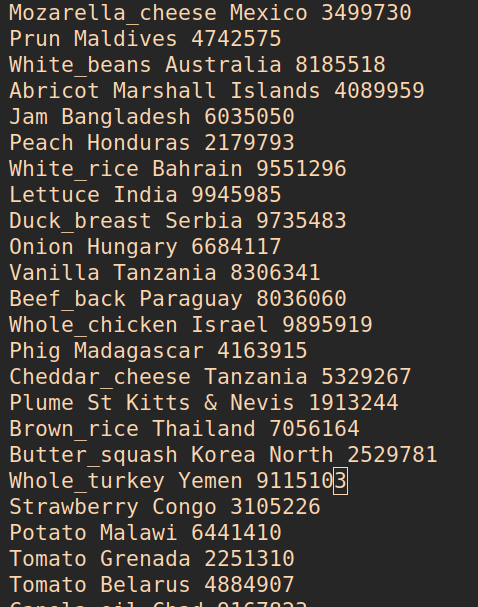
\includegraphics[width=0.7\textwidth]{pictures/test_file.png}
  \caption{Пример сгенерированного входного файла}
  \label{fig:test_file}
\end{figure}

\subsection{Алгоритм внешней сортировки "прямое слияние"}
\paragraph{Описание алгоритма}
Внешняя сортировка прямого слияния требует наличие нескольких
вспомогательных файлов (в нашем случае двух).
Каждый шаг сортировки состоит из фазы разделения
и слияния.

Разделение предполагает разбиение текущей последовательности на
несколько подпоследовательностей (порций) и поочередную запись в вспомогательные
файлы. Количество элементов в порции на каждом этапе увеличивается в 2
раза.

Слияние состоит в чтении вспомогательных файлов и упорядочивании
соответствующих порций. Для каждой порции сравниваются 2 записи, меньшая
из них записывается в исходный файл, и считывается новая запись из файла, в
котором содержалась меньшая. При достижении конца порции одного файла
оставшиеся записи другого файла переносятся без изменений. Данные
операции повторяются пока не будет достигнут конец одного из файлов, после чего
переписываются незатронутые записи из другого.
\paragraph{Код сортировки}
\lstinputlisting[firstline=1, lastline=130]{code/external_sorts.cpp}
\paragraph{Тестирование алгоритма}
Для тестирования алгоритма использовался класс TimeCounter.
\lstinputlisting[firstline=45, lastline=80]{code/sort_utilities.cpp}
Также использовалась отладочная версия данной сортировки.
\lstinputlisting[firstline=131, lastline=256]{code/external_sorts.cpp}
Результаты тестирования алгоритма на файле из миллиона записей можно
увидеть на рисунке \ref{fig:first_sort_test}.
\begin{figure}[htpb]
  \centering
  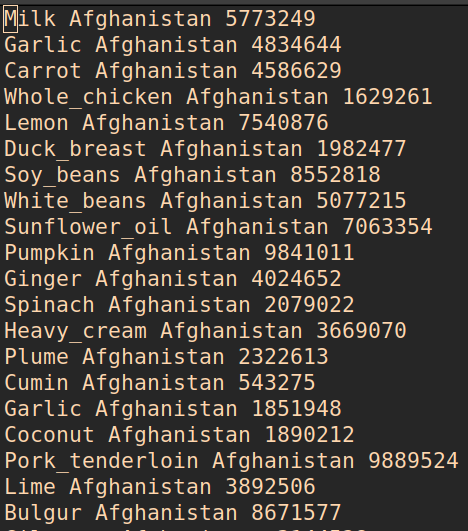
\includegraphics[width=0.7\textwidth]{pictures/first_sort_test.png}
  \caption{Первые строки файла после применения сортировки прямого слияния}
  \label{fig:first_sort_test}
\end{figure}

\newpage
\paragraph{Сводная таблица тестирования}
\begin{figure}[htpb]
  \centering
  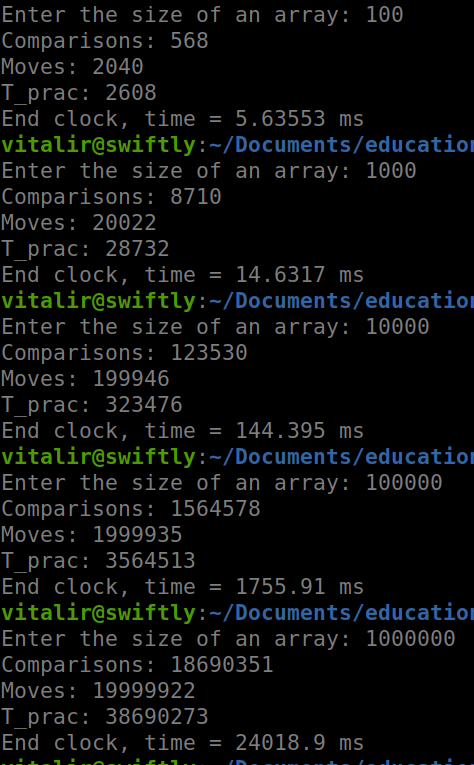
\includegraphics[width=0.45\textwidth]{pictures/first_sort_table.png}
  \caption{Результаты тестирования сортировки слиянием}
  \label{fig:first_sort_speed}
\end{figure}
\begin{table}[htpb]
  \centering
  \caption{Сводная таблица тестирования сортировки прямым слиянием}
  \label{tab:first_sort_speed}
  \begin{tabular}{|c|c|c|c|}
    \hline
    n & $T(n)$ & $T_\textup Т=f(C+M)$ &
    $T_\textup п=C_\textup ф+M_\textup ф$
    \\ \hline
    100
    & 5.63553 мс
    & \multirow{5}*{\centering $\Theta(n\log n)$}
    & 2608
    \\ \cline{1-2}\cline{4-4}
    1000
    & 14.6317 мс
    &
    & 28732
    \\ \cline{1-2}\cline{4-4}
    10000
    & 144.395 мс
    &
    & 323476
    \\ \cline{1-2}\cline{4-4}
    100000
    & 1755.91 мс
    &
    & 3564513
    \\ \cline{1-2}\cline{4-4}
    1000000
    & 24018.9 мс
    &
    & 38690273
    \\ \hline
  \end{tabular}
\end{table}

\newpage
\section{Задание 2}

\subsection{Постановка задачи}
Реализовать алгоритм внешней сортировки «естественное слияние» для
данных, в соответствии с персональным вариантом (указан в постановке
задачи задания No1).
\subsection{Алгоритм внешней сортировки "естественное слияние"}
\paragraph{Описание сортировки}
Внешняя сортировка естественного слияния работает над упорядоченными
последовательностями – сериями. Фазы разделения и слияния осуществляются
над сериями, не всегда имеющими одинаковый размер (в отличие от прямого
слияния).

Фаза разделения включает поиск и попеременную запись серий
максимальной длины из исходного файла в вспомогательные. Процедура
повторяется до конца файла.

Фаза слияния включает упорядочивание серий, получаемых из
вспомогательных файлов. Алгоритм фазы слияния идентичен сортировке
прямого слияния. В итоге, из двух серий образуется одна, она и является
отсортированной последовательностью.
\paragraph{Код сортировки}
\lstinputlisting[firstline=262, lastline=376]{code/external_sorts.cpp}
\paragraph{Тестирование алгоритма}
Для тестирования алгоритма использовался класс TimeCounter (код представлен в задании 1).
Также использовалась отладочная версия данной сортировки.
\lstinputlisting[firstline=382, lastline=477]{code/external_sorts.cpp}
Результаты тестирования алгоритма на файле из миллиона записей можно
увидеть на рисунке \ref{fig:second_sort_test}.
\begin{figure}[htpb]
  \centering
  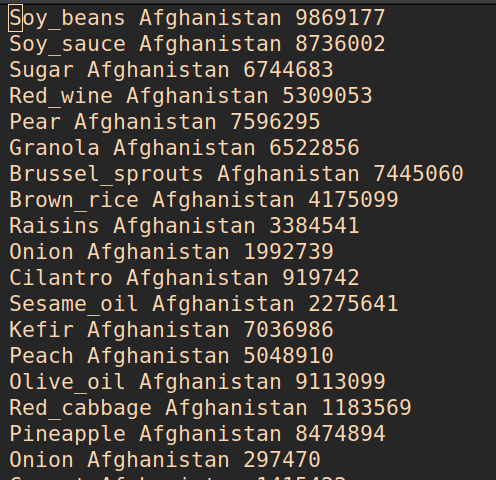
\includegraphics[width=0.7\textwidth]{pictures/second_sort_test.png}
  \caption{Первые строки файла после применения сортировки естественного слияния}
  \label{fig:second_sort_test}
\end{figure}

\newpage
\paragraph{Сводная таблица тестирования}
\begin{figure}[htpb]
  \centering
  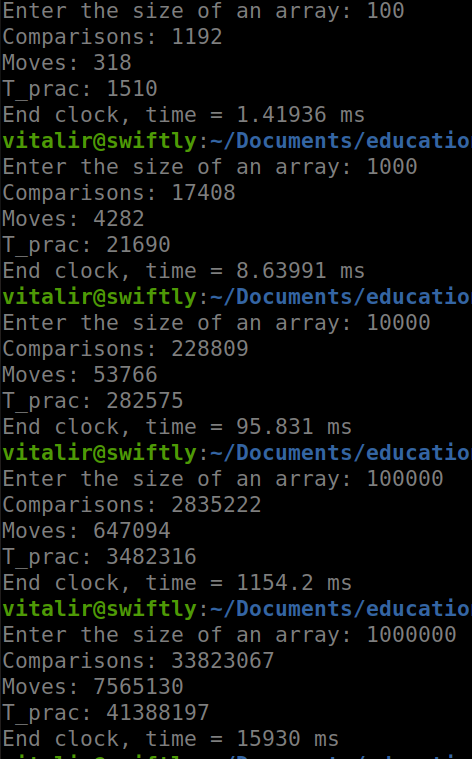
\includegraphics[width=0.45\textwidth]{pictures/second_sort_table.png}
  \caption{Результаты тестирования сортировки естественного слияния}
  \label{fig:second_sort_speed}
\end{figure}
\begin{table}[htpb]
  \centering
  \caption{Сводная таблица тестирования сортировки естественным слиянием}
  \label{tab:second_sort_speed}
  \begin{tabular}{|c|c|c|c|}
    \hline
    n & $T(n)$ & $T_\textup Т=f(C+M)$ &
    $T_\textup п=C_\textup ф+M_\textup ф$
    \\ \hline
    100
    & 1.41936 мс
    & \multirow{5}*{\centering $\Theta(n\log n)$}
    & 1510
    \\ \cline{1-2}\cline{4-4}
    1000
    & 8.63991 мс
    &
    & 21690
    \\ \cline{1-2}\cline{4-4}
    10000
    & 95.831 мс
    &
    & 282575
    \\ \cline{1-2}\cline{4-4}
    100000
    & 1154.2 мс
    &
    & 3483216
    \\ \cline{1-2}\cline{4-4}
    1000000
    & 15930 мс
    &
    & 41388197
    \\ \hline
  \end{tabular}
\end{table}

\newpage
\section*{Выводы}
\addcontentsline{toc}{section}{Выводы}
В ходе выполнения работы были реализованы алгоритмы внешних
сортировок "прямое слияние" и "естественное слияние". Исходя из времени
выполнения алгоритмов на больших входных данных на одной и той же машине,
алгоритм сортировки "естественное слияние" намного быстрее алгоритма
"прямое слияние" несмотря на одинаковую
вычислительную и емкостную сложность: $\Theta(n\log n)$ и $O(n)$ соответственно.
Это объясняется тем, что в алгоритме "естественное слияние" задействован
также и алгоритм внутренней сортировки, который работает значительно
быстрее за счет работы с внутренней памятью (т.к. на работу с устройствами
внешней памяти тратится значительное время по сравнению с внутренними). Из этого
также можно заметить зависимость скорости работы алгоритма
от размера данных, которые хранятся во внутренней памяти: чем больше таких
данных и меньше внешних, тем быстрее работает алгоритм.

\section*{Список информационных источников}
\addcontentsline{toc}{section}{Список информационных источников}
\begin{enumerate}[leftmargin=*] % delete left margin
  \item Thomas H. Cormen, Clifford Stein и другие: Introduction to Algorithms, 3rd Edition.
    Сентябрь 2009. The MIT Press.
  \item B. Strousrup: A Tour of C++ (2nd Edition). Июль 2018. Addison-Wesley.
  \item Quick sort~//~Wikipedia \\~
    [Электронный ресурс]. URL:
    \\ https://en.wikipedia.org/wiki/Quick\_sort
    (Дата обращения: 26.04.2021)
  \item Jon Bentley, Douglas McILROY: Engineering a sort function. Ноябрь 1993.
    John Wiley \& Sons.
   \item Курс Algorithms, part 1 // Coursera [Электронный ресурс]. URL:
     \\ https://www.coursera.org/learn/algorithms-part1
     (Дата обращения: 26.04.2021)
\end{enumerate}

\end{document}
